% $Id: intro.tex,v 1.1.1.1 2007/10/03 22:28:18 hridesh Exp $

\section{Introduction}
For this course project, I extended the lambda calculus language with the generator feature for memory efficiency in iteration operations.

\subsection{Motivation}
Generator functions can generate a function that behaves like an iterator. They allow programmers to make an iterator in a fast, easy and clean way without too much memory cost. To illustrate this, let us consider a simple Python example of building a list and return it\cite{generators}.
%
\begin{figure}[H]
	\centering
	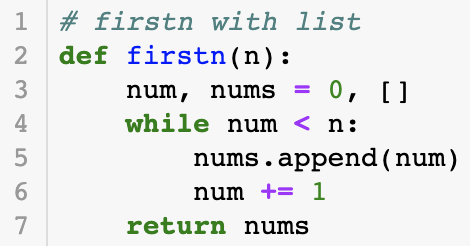
\includegraphics[width=0.4\textwidth]{figures/fstn}
	\caption{Firstn with List}
\end{figure}
%
In figure 1, the function firstn return a full list with length n in memory. If n is really big number and each integer keeps 10 megabyte in memory, then we need to cost a lot of memory to extend our RAM.
%
\begin{figure}[H]
	\centering
	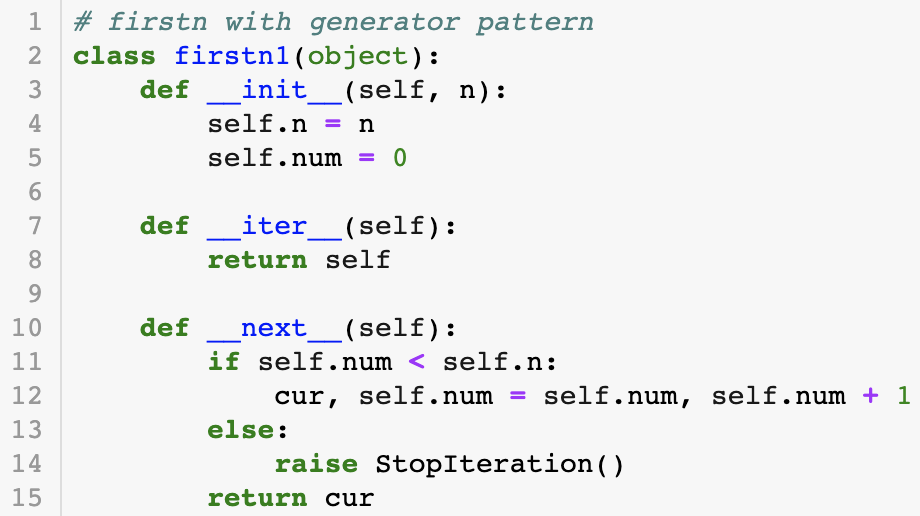
\includegraphics[width=0.75\textwidth]{figures/fstn1}
	\caption{Firstn with List}
\end{figure}
%
To save memory space, we can implement the firstn1 as an object with generator pattern, fig 2. Class firstn1 is iterable and it will perform as we expect. However, we need to write a bunch lines of code to implement it and the logic is expressed in a convoluted way.

%
\begin{figure}[H]
	\centering
	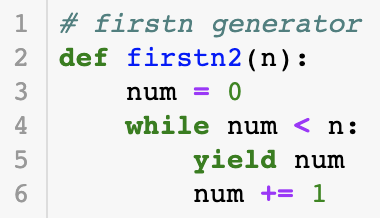
\includegraphics[width=0.4\textwidth]{figures/fstn2}
	\caption{Firstn Generator}
\end{figure}
%

Python provides generator feature in each functions. In the figure 3, the keyword \textit{yield} indicates that the function firstn2 is a generator that yields items in the iteration instead of returning a list. Compare the actually object sizes in these approaches with the same input 10k. The figure 4 shows that the generator has a huge advantage not only in memory efficiency but also in clear and natural logic. 

%
\begin{figure}[H]
	\centering
	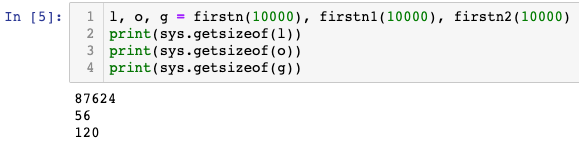
\includegraphics[width=0.75\textwidth]{figures/memsize}
	\caption{Memory Sizes}
\end{figure}
%

\subsection{Background}
In this section, I will show necessary background about this generator functions. For ordinary functions, they have a single entry point and multiple exit points(return statements). When we call a function, the code runs from the first line of the function until it finds an exit point. After that, the function's stack of local variables are cleared and the corresponding memory reclaimed by the OS\cite{magic}.

However, the generator function have multiple entry and exit points. The function's stack of local variables are allocated on heap memory instead of stack memory. Each \textit{yield} statement will defines an exit point and a re-entry point in the same location. The generator function runs until a \textit{yield} statement is encountered. At that point, the function is paused. And the flow of control is yielded to the caller of the generator function and then back to the re-entry point to resume the function. 

\begin{figure}[H]
	\centering
	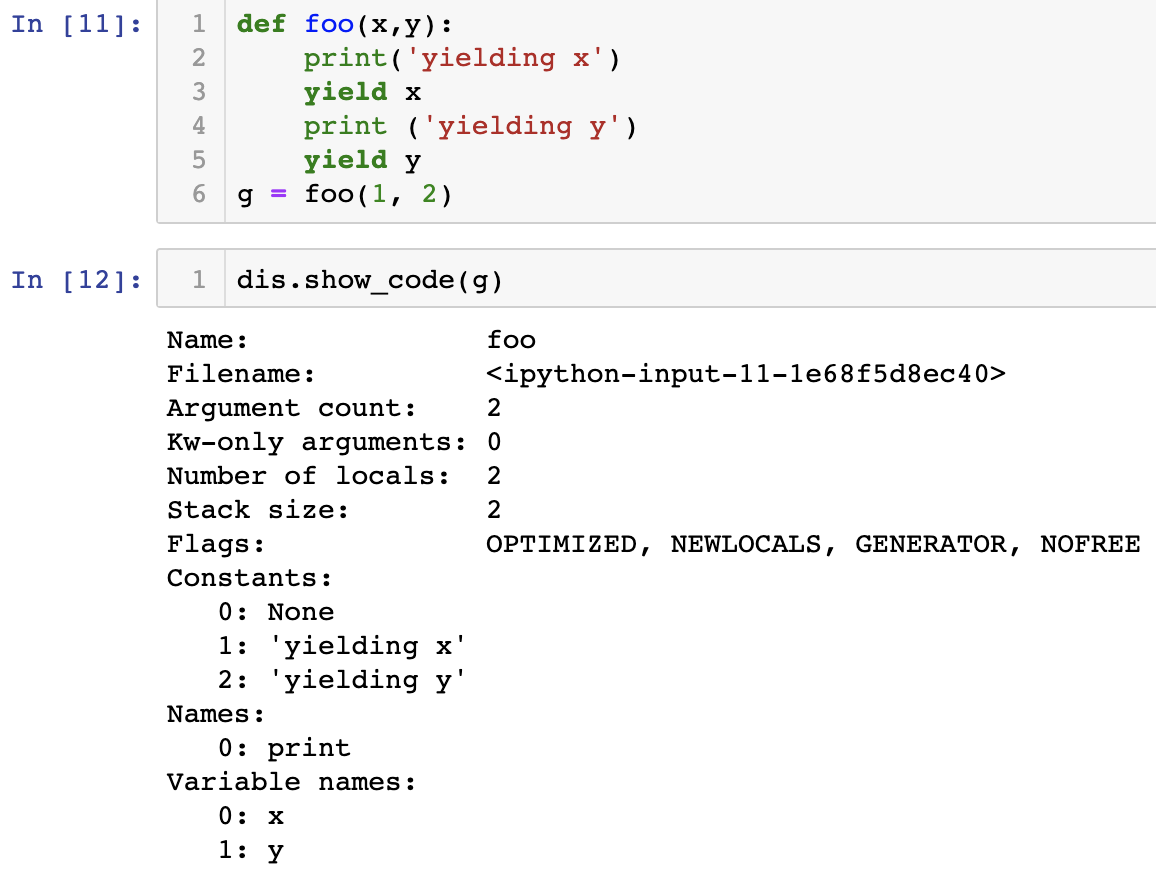
\includegraphics[width=0.75\textwidth]{figures/foo1}
	\caption{Function \textit{foo} with Yield}
\end{figure}

In the figure 5, variable \textit{g} indicates the generator \textit{foo(1, 2)}. When the CPython compiler finds the \textit{yield} keyword in a function, it sets a GENERATOR flag. Then, the compiler returns a generator object which is iterable. If we apply \textit{next} function with the generator, then it returns the values of variable \textit{x, y} in the first two calls respectively as shown in Figure 6.

\begin{figure}[H]
	\centering
	\subfloat[Before Next]{{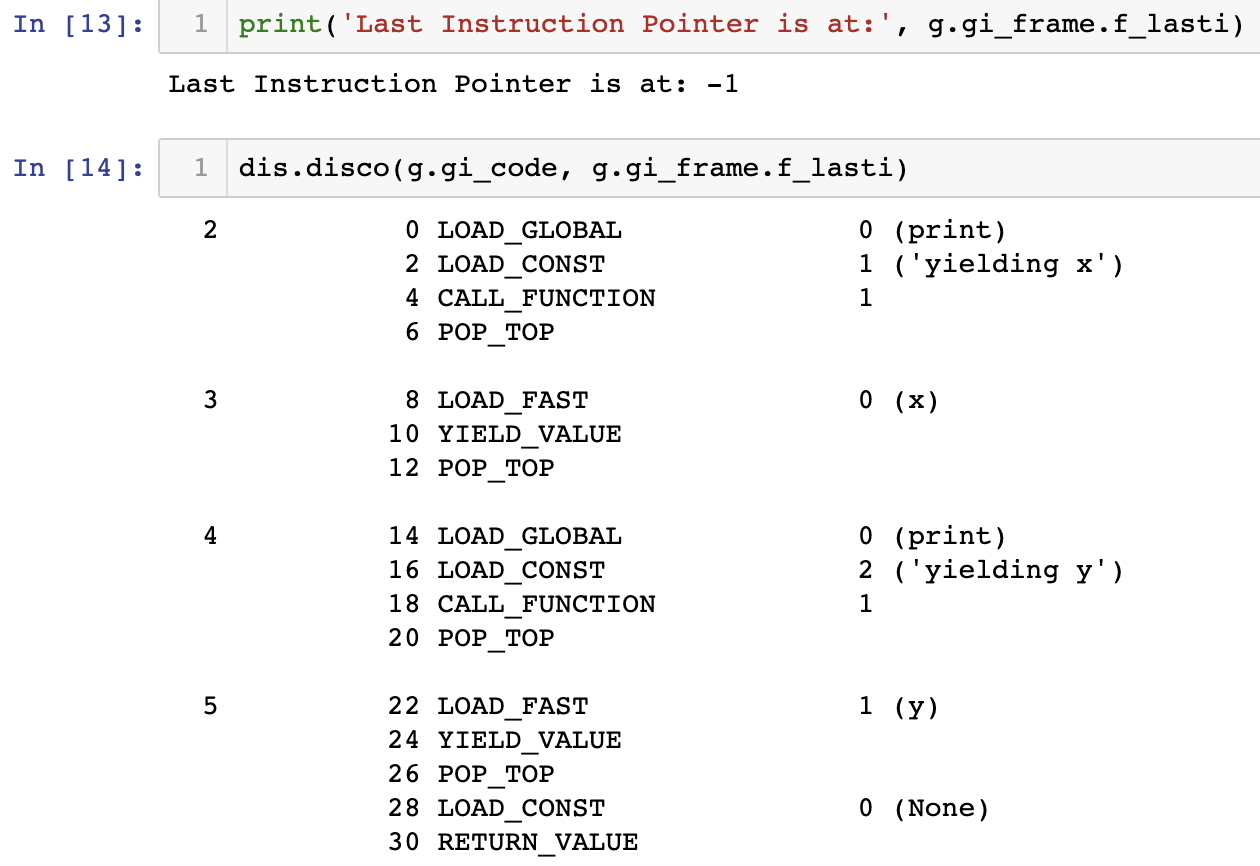
\includegraphics[width=5cm]{figures/foo2} }}%
	\qquad
	\subfloat[First Next]{{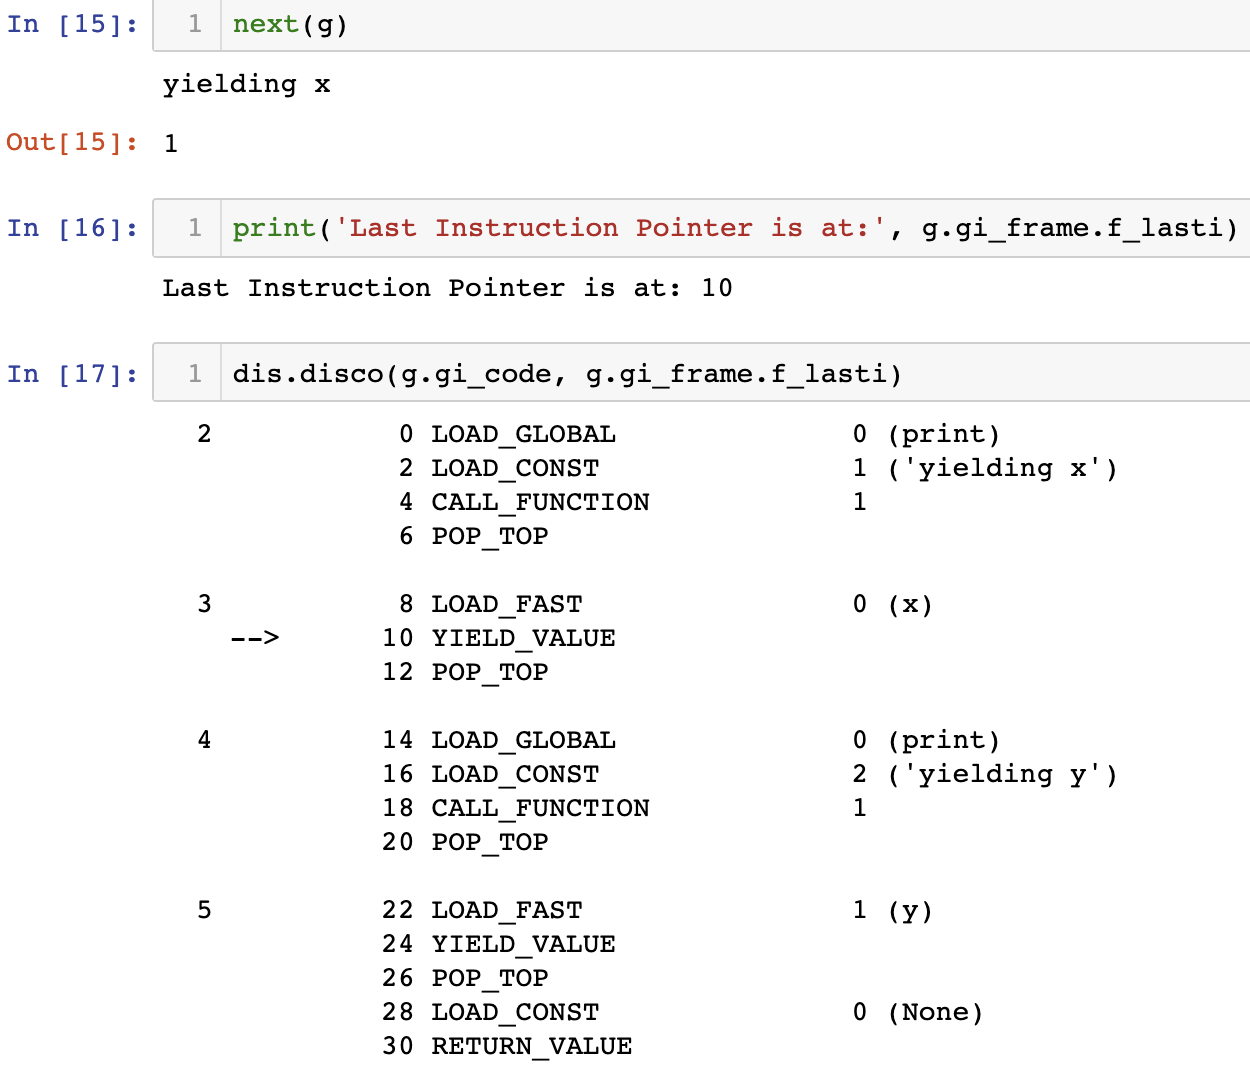
\includegraphics[width=5cm]{figures/foo3} }}%
	\qquad
	\subfloat[Second Next]{{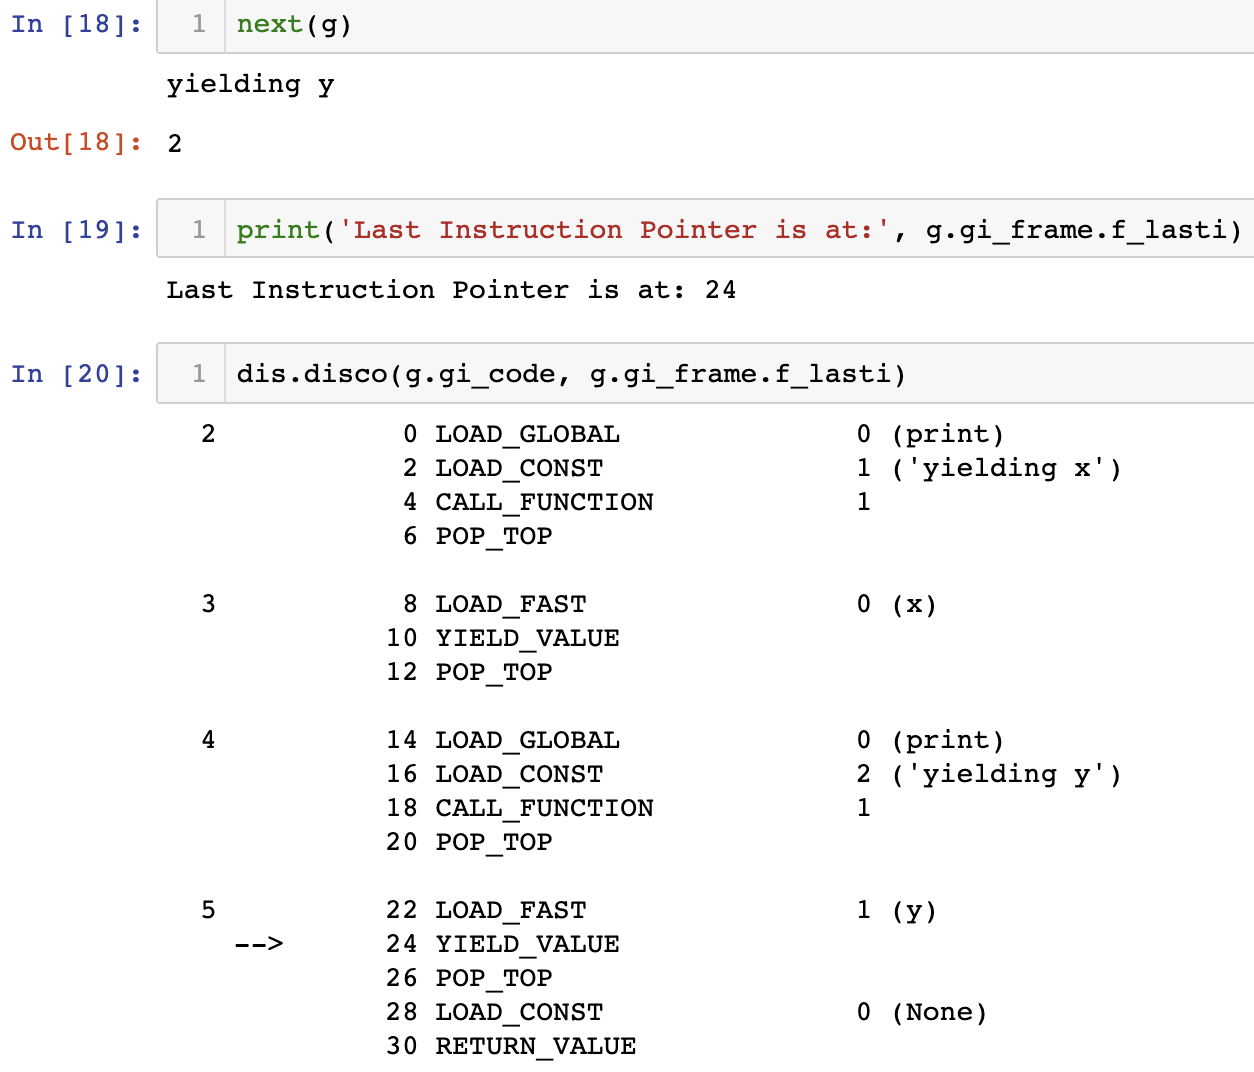
\includegraphics[width=6cm]{figures/foo4} }}%
	\caption{Iterable Generator Foo}%
	\label{fig:example}%
\end{figure}

